\chapter{Implementation}  \label{Chapter:Implementation}

My implementation of software project telemetry has been integrated into the Hackystat system. Hackystat is an open-source framework developed in the Collaborative Software Development Lab (CSDL) at the University of Hawaii for automated collection and analysis of software product and process metrics and empirical software engineering experimentation. I have been contributing to its development since 2002. The relationship between my implementation of software project telemetry and Hackystat is illustrated in Figure \ref{fig:TelemetryImplementation}.
The implementation can be viewed as an extension to the Hackystat framework. CSDL members often use ``Hackystat'' as an umbrella term to refer to the framework plus all the extensions built on top of it. However, for the purpose of clarity, I will try to make a distinction between them. Throughout this chapter:

\begin{itemize}
	\item The \textit{``Hackystat framework''} refers to the core framework components that provide metrics storage service and extension plug-in mechanism.
	\item The \textit{``software project telemetry''} refers my implementation of software project telemetry.
	\item The \textit{``Hackystat system''} refers to the framework plus all the extensions built on top of it.
\end{itemize}

\begin{figure}[p]
  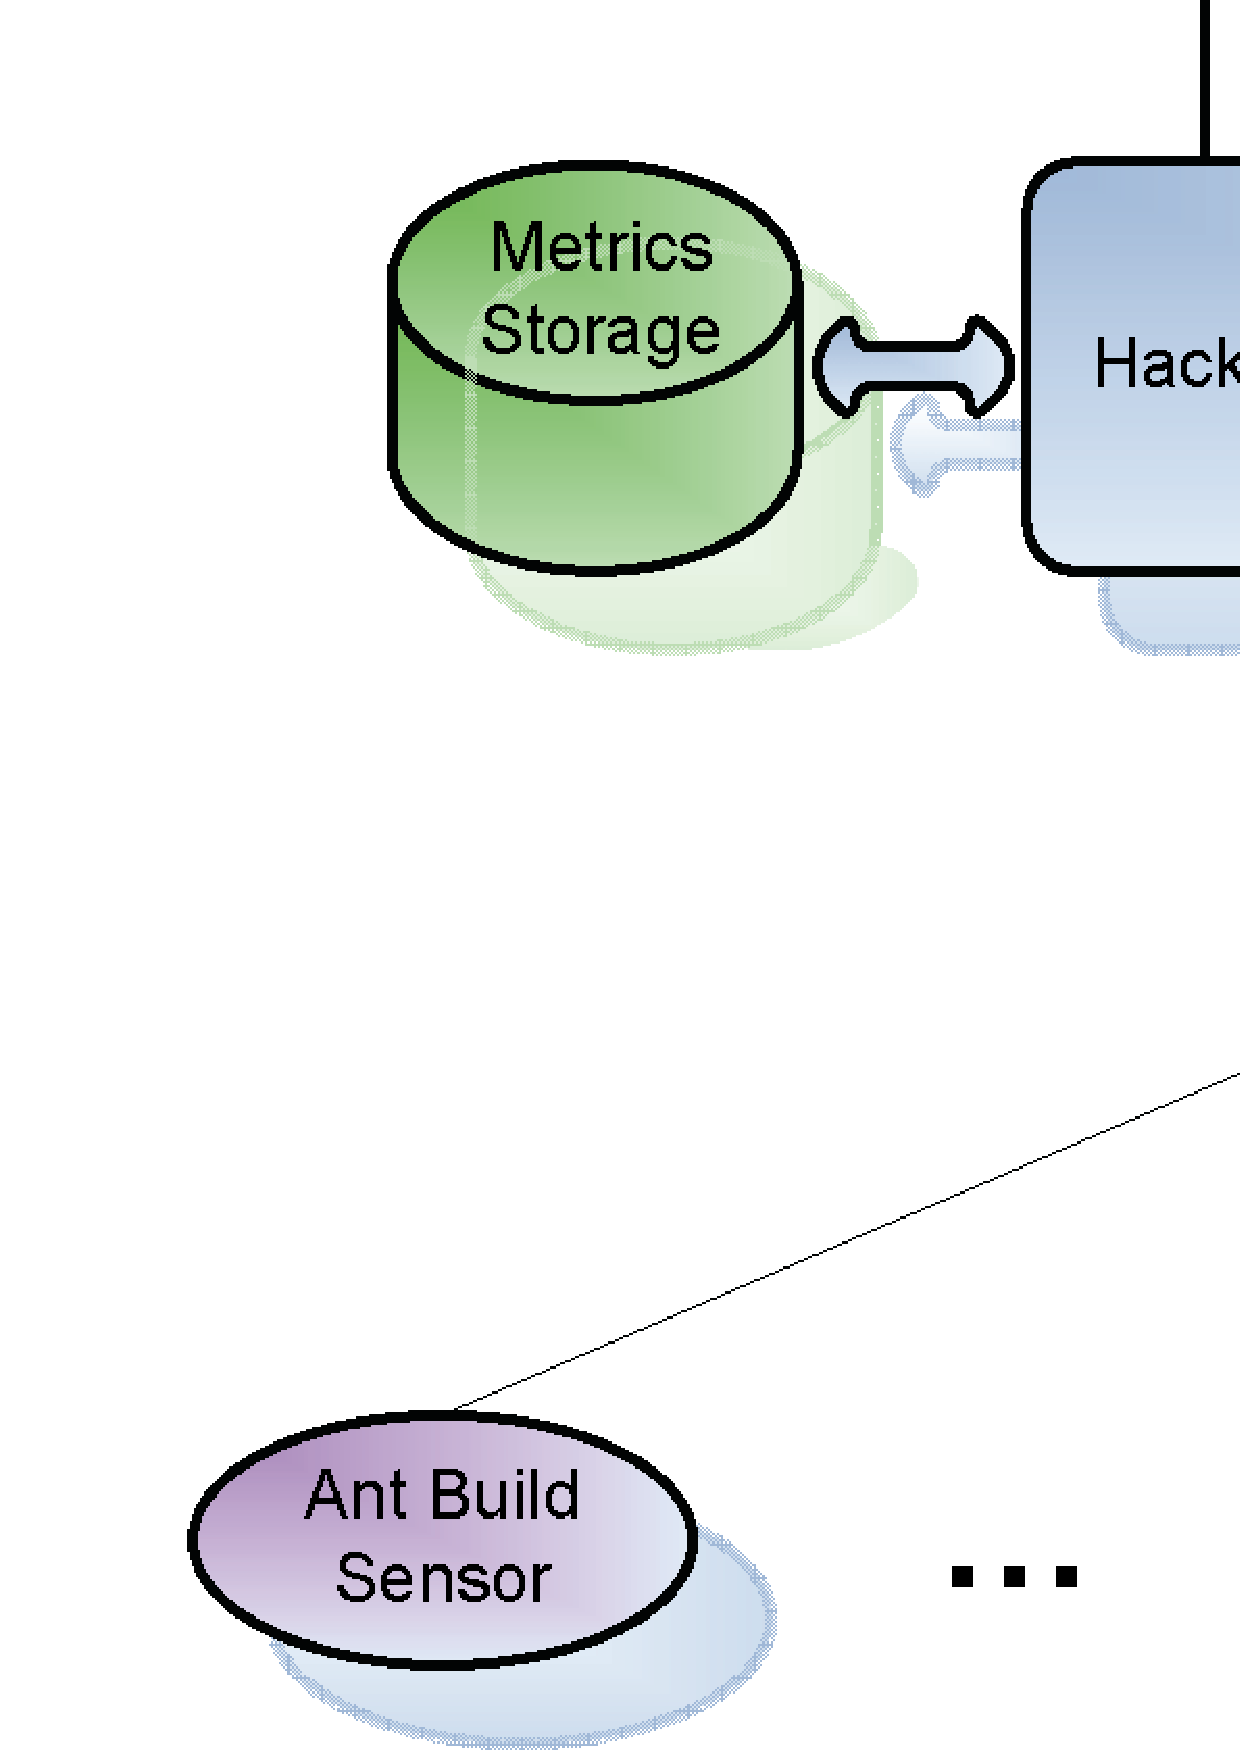
\includegraphics[width=1.00\textwidth]{figures/TelemetryImplementation}
  \caption{Software Project Telemetry System Implementation} 
  \label{fig:TelemetryImplementation}
\end{figure}

This chapter starts with a brief overview of the Hackystat framework and the services it provides in Section \ref{Implementation:Hackystat}. 
Section \ref{Implementation:Telemetry} describes my implementation of software project telemetry, which utilizes Hackystat framework services.
Section \ref{Implementation:ReducersFunctions} introduces all available telemetry \textit{reducers} and \textit{functions}.
Section \ref{Implementation:Summary} summarizes this chapter.







%%%%%%%%%%%%%%%%%%%%%%%%%%%%%%%%%%%%%%%%%%%%%%%%%%%%%%%%%
%                                                       %
%                   S E C T I O N                       %
%                                                       %
%%%%%%%%%%%%%%%%%%%%%%%%%%%%%%%%%%%%%%%%%%%%%%%%%%%%%%%%%

\section{Hackystat Framework} \label{Implementation:Hackystat}

Hackystat is an open-source framework developed in the Collaborative Software Development Lab (CSDL) at the University of Hawaii for automated collection and analysis of software product and process metrics and empirical software engineering experimentation. 
The framework itself is tool, environment, process, and application independent. It does not presume a specific operating system platform, a specific integrated development environment, a specific software process, or a specific application area. It is designed to be extended. Therefore, it only provides generic services such as metrics storage, project definition management, and an extension mechanism where new modules (functionalities) can be plugged in.

A Hackystat system is configured from a set of modules, which determine the actual functionality of the system: which development tools are supported, what types of software metrics are collected, and what analyses are run on the metrics. For example, several different research projects are being conducted using Hackystat. One research involves a Hackystat system configured from a set of modules specialized in low-level software process analysis \cite{Kou:2006}. Another research involves another Hackystat system configured from another set of modules trying to understand parallel software development for high performance computers \cite{Johnson:2005}. This thesis reports on my research involving yet another Hackystat system configured from yet another set of modules supporting project management and process improvement.




%%%%%%%%%%%%%%% S U B  S E C T I O N %%%%%%%%%%%%%%%%%%%%
\subsection{Metrics Storage}

The Hackystat framework exposes two interfaces related to metrics storage as illustrated in Figure \ref{fig:TelemetryImplementation}: one for metrics data reception, and the other for metrics retrieval.

The metrics data reception interface is used by sensors to send software process and product metrics. The communication occurs on an HTTP SOAP channel. Hackystat developers often refer to the Hackystat architecture as a client-server system. In this view, the \textit{``clients''} are development environment tools, such as editors (Emacs, Eclipse, Vim), configuration management systems (CVS, Harvest), build tools (Ant, Make), unit testing tools (JUnit), and so forth. For each of these tools, a custom sensor must be developed. The \textit{``server''} refers to the Hackytat framework kernel plus all the analysis extensions. They run inside a standard J2EE\footnote{J2EE stands for Java 2 Platform Enterprise Edition. Starting from version 5, Sun Microsystem has re-branded it as Java EE.} application container.

The metrics retrieval interface is used by metrics analysis extensions on the server side. Strictly speaking, the analysis code might opt not to use this interface directly. Instead, it may choose to rely on a higher level metrics abstraction mechanism which in turn depends on the metrics retrieval interface.

The Hackystat framework kernel handles metrics data storage automatically. The persistence engine is completely opaque, visible neither to the client-side sensors nor to the server-side analysis code. The current kernel implementation stores all metrics data in plain file system files in XML format. 



%%%%%%%%%%%%%%% S U B  S E C T I O N %%%%%%%%%%%%%%%%%%%%
\subsection{Project Definition Management} 

Sensors simply send bits of raw data concerning software process or product to the server. They know nothing about the larger context in which the development is performed. For example, during a typical day, a developer might work on several distinct tasks: an hour in the morning on requirements for an upcoming project, and two hours in the afternoon on maintenance fixes to an old system. For the requirements project, the developer is working in a team with one other person; while the system maintenance and development involves 12 people. In most cases, the developer will want to analyze the requirements data separately from the maintenance data. The developer will also probably want to gain a higher level perspective on the progress of the requirements project by combining his data and the relevant data from the other person he is working with. Similarly, it would be helpful to combine together the relevant data from all the 12 people working on maintenance to see how that project is progressing.
 
The Hackystat framework kernel supports team level analysis through project definitions. The project definition is designed to specify a context for analysis of sensor data, including the set of workspaces containing the artifacts associated with the project, the set of Hackystat users who are participating in the project and whose metrics should be combined together, and the time period during which the project is underway.




%%%%%%%%%%%%%%% S U B  S E C T I O N %%%%%%%%%%%%%%%%%%%%
\subsection{Extension Mechanism}

A Hackystat system provides all end user functionalities through extension modules. The framework exposes \textit{``extension points''} to support extensions along multiple dimensions including sensors, metrics types, metrics analysis, documentation, and so forth. For each new functionality, the framework requires the developer to specify a declaration file in XML format to supply information about the specific extension implemented. Detailed information about the extension points is available in the Hackystat developer documentation, which can be found at the Hackystat home page: \textit{www.hackystat.org}. 






%%%%%%%%%%%%%%%%%%%%%%%%%%%%%%%%%%%%%%%%%%%%%%%%%%%%%%%%%
%                                                       %
%                   S E C T I O N                       %
%                                                       %
%%%%%%%%%%%%%%%%%%%%%%%%%%%%%%%%%%%%%%%%%%%%%%%%%%%%%%%%%

\section{Hackystat Telemetry Module} \label{Implementation:Telemetry}

The core of my implementation of software project telemetry resides in a Hackystat extension module called \textit{``Core\_Telemetry''}. It contains about 15,000 lines of code. The module itself is extensible to accommodate new metrics types and analyses that might arise in the future. It exposes two extension points of its own, where custom implementation of \textit{telemetry reducers} and \textit{telemetry functions} can be plugged in. 

Just like the functionality of a Hackystat system is determined by its constituent modules, the functionality of the telemetry module hinges on the availability of reducers and functions. I have implemented over a dozen reducers and several functions to support this thesis research. They are distributed in the Hackystat modules where different types of software metrics are defined. They constitute about 13,000 lines of code. Available reducers and functions are listed in Section \ref{Implementation:ReducersFunctions}.



\subsection{Functional Description} \label{Implementation:Telemetry:FunctionalDescription}

The software project telemetry implementation provides three analyses where a user can perform telemetry related exploration. 

\begin{figure}[tbp]
  \includegraphics[width=1.00\textwidth]{figures/TelemetryDefinitionManagement}
  \caption{Telemetry Definition Management Console} 
  \label{fig:TelemetryDefinitionManagement}
\end{figure}

\begin{itemize}
	\item \textbf{Telemetry Expert Analysis} --- 
Figure \ref{fig:TelemetryExpertAnalysis} is a screenshot of the telemetry expert analysis. The user uses telemetry language to interact with the system directly to explore trends and relationships between different software product and process metrics. This is the most powerful and flexible analysis, and the user has the finest control.
%from determining which metrics to use and how to manipulate them, to the display details of the chart.
The expert analysis is especially useful when a user is experimenting with different forms of telemetry streams. Once the user is satisfied with the generated chart or report, he can create a persistent definition through the telemetry definition management console, so that later invocation of the same analysis can be performed through the telemetry chart/report analysis saving the effort of typing the definition again. Figure \ref{fig:TelemetryDefinitionManagement} is a screen shot showing a user creating a persistent definition of a telemetry chart with the definition management console.
	
	\item \textbf{Telemetry Report Analysis} --- 
Figure \ref{fig:TelemetryReportChartStream} is a screenshot of the telemetry report analysis.
This analysis performs the same analysis as the telemetry expert analysis, except that it hides the telemetry language from the end user. Instead of typing telemetry definitions directly, a user selects a predefined telemetry report from a drop-down list and performs the analysis.
The telemetry definition management console shown in Figure \ref{fig:TelemetryDefinitionManagement} allows a system administrator or a telemetry expert to define a set of commonly used telemetry charts and reports and made them available in the drop-down box that the end user sees.	This is a good way to lower the adoption barrier of software project telemetry, because it eliminates the need for a normal user to learn the telemetry language.
	
	\item \textbf{Telemetry Chart Analysis} ---
The telemetry chart analysis is similar to the telemetry report analysis. The only different is that the report analysis generates a group of related charts, while the chart analysis generates one single chart.

\end{itemize}








\subsection{Implementation Details}

The core of software project telemetry implementation resides in a Hackystat extension module called \textit{``Core\_Telemetry''}. The package structure is illustrated in Figure \ref{fig:TelemetryPackageStructure}. It includes the following components:

\begin{itemize}
	\item \textbf{Telemetry Language Parser} --- 
The telemetry language parser parses user input of telemetry definitions into an abstract syntax tree, which is a Java object representation of telemetry definitions. The formal grammar of the telemetry language is specified in Appendix \ref{Chapter:TelemetryLanguageSpecification}. Figure \ref{fig:TelemetryAST} is a UML diagram for static structure of the telemetry abstract syntax tree. Internally, the parser is generated using JavaCC \cite{Software:JavaCC}: a top-down Java parser generator.

	\item \textbf{Telemetry Streams Data Model} ---
This is the data model for telemetry streams. It contains computed values ready to be rendered or displayed to the end user.

	\item \textbf{Telemetry Reducers}\footnote{Telemetry reducers are also known as telemetry reduction functions, because the grammar to invoke a telemetry reducer is the same as the grammar to invoke a telemetry function. However, the similarity is superficial since the underlying implementation is completely different.} ---
This package contains the telemetry reducer extension point. A telemetry reducer aggregates low level software product and process data, and returns a collection of telemetry streams. To provide a custom implementation, a developer has to implement the \textit{``TelemetryReducer''} interface and supply a declaration file in XML format. The Core\_Telemetry module uses Java reflection to discover and load custom reducer implementations dynamically at runtime. 
	
	\item \textbf{Telemetry Functions}\footnote{This definition excludes telemetry reduction functions.} ---
This package contains the telemetry function extension point. A telemetry function takes a telemetry stream collection as input, and returns another telemetry streams collection as output. To provide a custom implementation, a developer has to implement the \textit{``TelemetryFunction''} interface and supply a declaration file in XML format. The Core\_Telemetry module uses Java reflection to discover and load custom function implementations dynamically at runtime. 
	
	\item \textbf{Telemetry Evaluation Engine} ---
The telemetry evaluation engine walks the telemetry abstract syntax tree, resolves references to telemetry definitions, and invokes telemetry reducers and functions. The evaluation result is either a telemetry chart or a telemetry report.
	
	\item \textbf{Telemetry Definition Management Console} ---
This package implements a web interface for the telemetry definition management console, which allows a user to manage persistent definitions of telemetry streams, charts, and reports. The persistent definitions are used by the telemetry chart/report analysis, so that a user can select from a list of predefined charts or reports to perform the analysis.

	\item \textbf{Telemetry Analysis} ---
This package implements the web UI for the three telemetry analyses introduced in Section \ref{Implementation:Telemetry:FunctionalDescription}: the expert analysis, the report analysis, and the chart analysis.
	
\end{itemize}



\begin{figure}[p]
  \includegraphics[width=1.00\textwidth]{figures/TelemetryPackageStructure}
  \caption{Core\_Telemetry Module Package Structure} 
  \label{fig:TelemetryPackageStructure}
\end{figure}


\begin{figure}[p]
  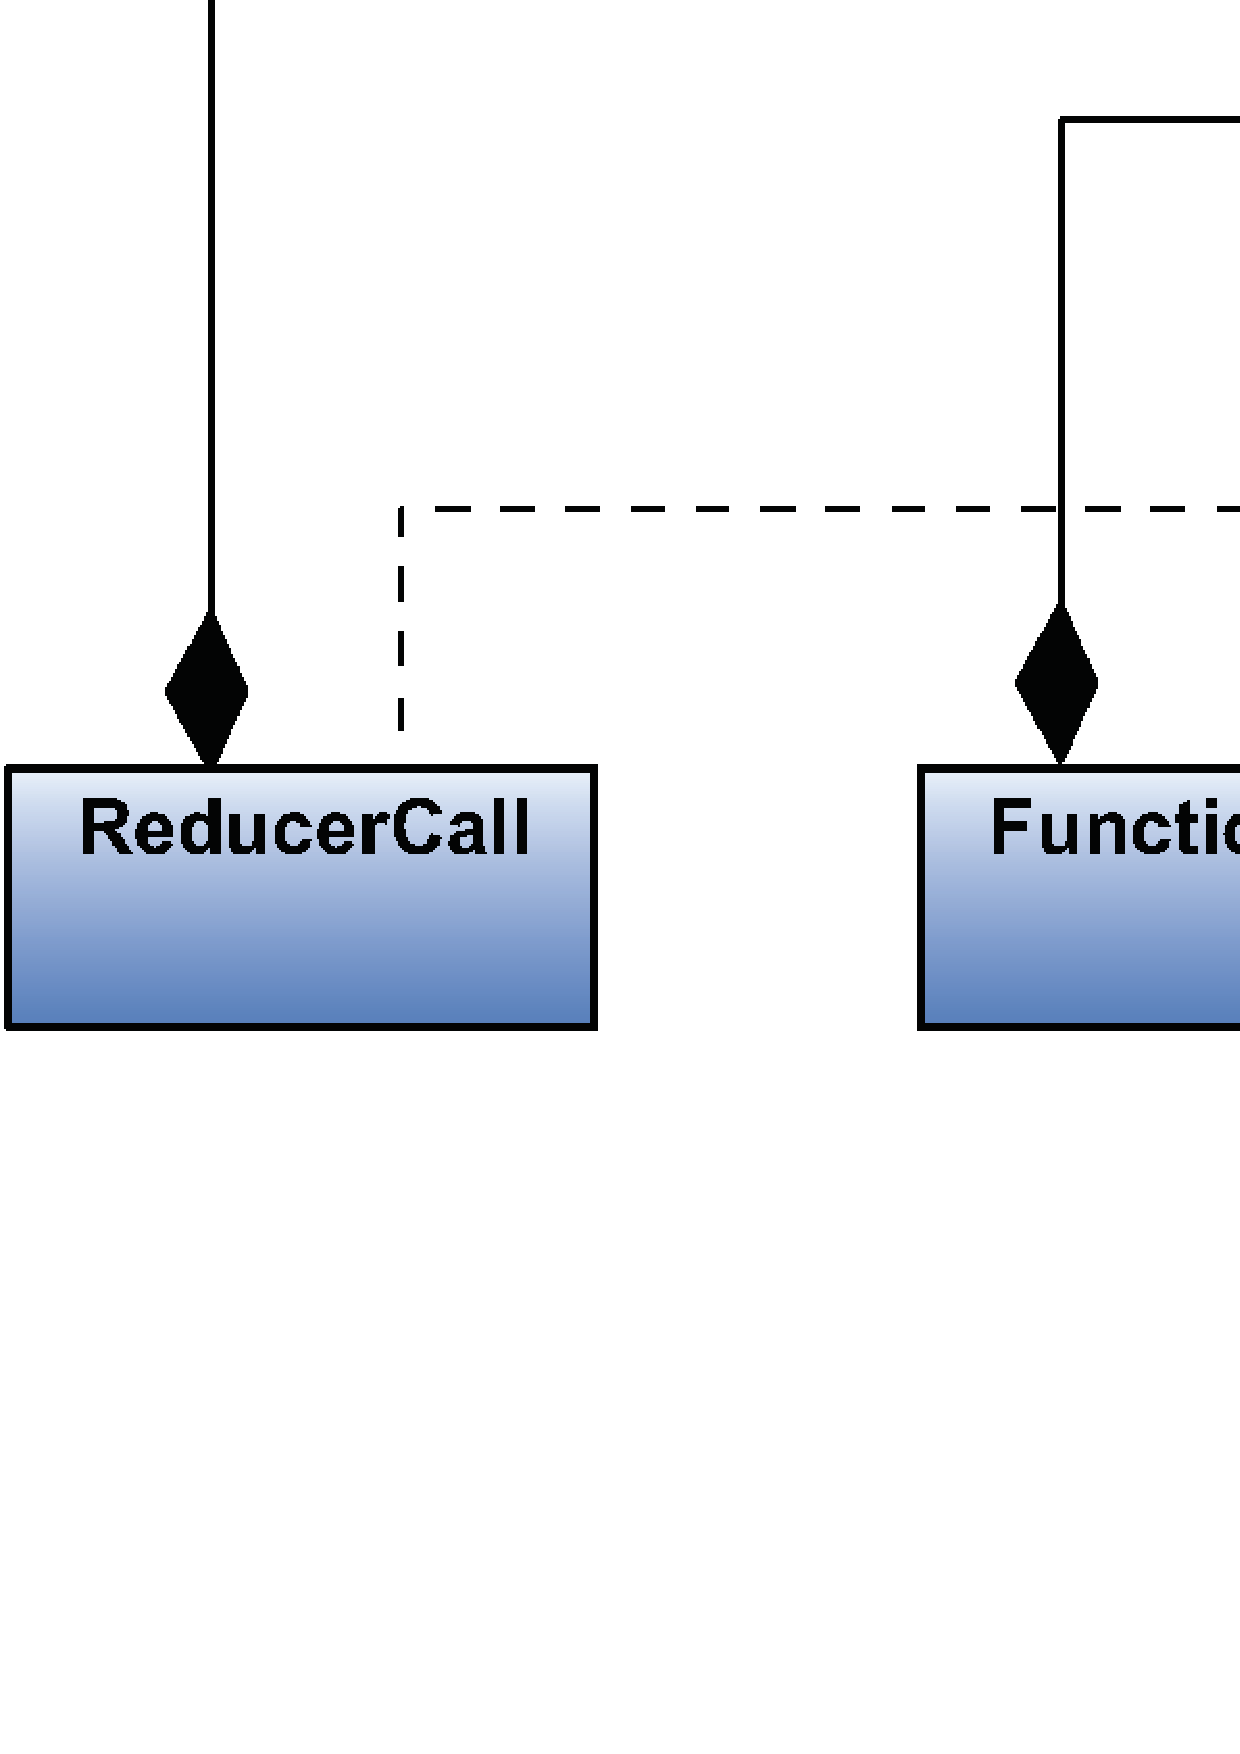
\includegraphics[angle=90, height=0.90\textheight]{figures/TelemetryAST}
  \caption{Telemetry Language Abstract Syntax Tree} 
  \label{fig:TelemetryAST}
\end{figure}










%%%%%%%%%%%%%%%%%%%%%%%%%%%%%%%%%%%%%%%%%%%%%%%%%%%%%%%%%
%                                                       %
%                   S E C T I O N                       %
%                                                       %
%%%%%%%%%%%%%%%%%%%%%%%%%%%%%%%%%%%%%%%%%%%%%%%%%%%%%%%%%
\newpage
\section{Telemetry Reducers and Functions} \label{Implementation:ReducersFunctions}

The Core\_Telemetry module is itself an extensible framework. It defines extension points for telemetry reducers and functions. The functionality of the telemetry module is determined by the available implementation of reducers and functions in a system. This section lists the reducers and functions that are currently available.







\subsection{Telemetry Reducers} \label{Implementation:Reducers}

The following telemetry reducers are available:

\begin{itemize}  
	\item \textbf{ActiveTime Reducer:}\\ 
Computes single telemetry stream for project active time in hours.
    
	\item \textbf{Build Reducer:}\\
Computes single telemetry stream for build success count or build failure count.

	\item \textbf{CodeChurn Reducer:}\\
Computes single telemetry stream for code churn: lines added or lines deleted.

	\item \textbf{CodeIssue Reducer:}\\
Computes single telemetry stream for the number of potential issues in the code generated by tools like FindBugs \cite{Software:FindBugs} and PMD \cite{Software:PMD}.

	\item \textbf{Commit Reducer:}\\
Computes single telemetry stream for code commit count.

	\item \textbf{CommitCycle Reducer:}\\
Computes single telemetry stream for the number of commits with specified local quality assurance behavior.

	\item \textbf{FileMetric Reducer:}\\
Computes single telemetry stream for source code size information.

	\item \textbf{IntegrationBuildFailure Reducer:}\\
Computes single telemetry stream for the number of integration build failures.

	\item \textbf{Issue Reducer:}\\
Computes single telemetry stream for the number of issues satisfying specified criteria.

	\item \textbf{JavaCoverage Reducer:}\\
Computes single telemetry stream for Java code unit test coverage.

	\item \textbf{JavaDependency Reducer:}\\
Computes single telemetry stream for Java code dependency.

	\item \textbf{LanguageFileMetric Reducer:}\\
Computes multiple telemetry streams for source code size information, one telemetry stream for each language found in the project.

	\item \textbf{MemberActiveTime Reducer:}\\
Computes multiple telemetry streams for member active time in hours, one telemetry stream for each member of the project.

	\item \textbf{MemberCodeChurn Reducer:}\\
Computes multiple telemetry streams for code churn, one telemetry stream for each member of the project.

	\item \textbf{MemberCommit Reducer:}\\
Computes multiple telemetry streams for code commit count, one telemetry stream for each member of the project.

	\item \textbf{MemberUnitTest Reducer:}\\
Computes multiple telemetry streams for the number of successful or failed unit test invocations, one telemetry stream for each member of the project.

	\item \textbf{Perf Reducer:}\\
Computes single or multiple telemetry streams for the values regarding a
performance test. Multiplicity is determined by reducer parameter values.

	\item \textbf{ReviewActivity Reducer:}\\
Computes single or multiple telemetry streams for project review active time in hours. Multiplicity is determined by reducer parameter values.

	\item \textbf{ReviewFile Reducer:}\\
Computes single or multiple telemetry streams for the number of files reviewed. Multiplicity is determined by reducer parameter values.

	\item \textbf{ReviewIssue Reducer:}\\
Computes single or multiple telemetry streams for the number of issues uncovered through code reviews. Multiplicity is determined by reducer parameter values.

	\item \textbf{UnitTest Reducer:}\\
Computes single telemetry stream for the number of successful or failed unit test invocations in the project.

	\item \textbf{WorkspaceActiveTime Reducer:}\\
Computes multiple telemetry streams for active time in hours in top level workspaces, one telemetry stream for each top level workspace.

	\item \textbf{WorkspaceCodeChurn Reducer:}\\
Computes multiple telemetry streams for code churn in top level workspaces, one telemetry stream for each top level workspace.

	\item \textbf{WorkspaceCommit Reducer:}\\
Computes multiple telemetry streams for code commit count in top level workspaces, one telemetry stream for each top level workspace.

	\item \textbf{WorkspaceCoverage Reducer:}\\
Computes single telemetry stream for Java code unit test coverage in top level workspaces, one telemetry stream for each top level workspace.

	\item \textbf{WorkspaceFileMetric Reducer:}\\
Computes multiple telemetry streams for source code size information in top level workspaces, one telemetry stream for each top level workspace.

\end{itemize}








\subsection{Telemetry Functions} \label{Implementation:Functions}

The following telemetry functions are available:

\begin{itemize}  
	\item \textbf{Add Function:}\\
Internal stock function supporting telemetry language operator ``+.''
	
	\item \textbf{Sub Function:}\\
Internal stock function supporting telemetry language operator ``-.''

	\item \textbf{Mul Function:}\\
Internal stock function supporting telemetry language operator ``*.''
	
	\item \textbf{Div Function:}\\
Internal stock function supporting telemetry language operator ``/.''

	\item \textbf{Filter Function:}\\
User callable function that filters out telemetry streams in a telemetry stream collection according to specified ranking function and threshold value.

	\item \textbf{FilterZero Function:}\\
Usable callable function that filters out telemetry streams with values of zero or no value in a telemetry stream collection.

\end{itemize}




%%%%%%%%%%%%%%%%%%%%%%%%%%%%%%%%%%%%%%%%%%%%%%%%%%%%%%%%%
%                                                       %
%                   S E C T I O N                       %
%                                                       %
%%%%%%%%%%%%%%%%%%%%%%%%%%%%%%%%%%%%%%%%%%%%%%%%%%%%%%%%%

\section{Chapter Summary} \label{Implementation:Summary}

In this chapter, I have introduced my implementation of software project telemetry. It is implemented as a Hackystat extension module. More detailed information and the source code are available at the Hackystat public website: \textit{www.hackystat.org}. The next chapter discusses the evaluation strategy for software project telemetry.

